
% ********** Chapter 9 **********
\chapter{Java ME Client}
\label{sec:JavaMEClient}

The Java ME Client is a client of web service interface which described in Chapter \nolinebreak \ref{sec:WebServiceInterface}. It implemented all of the interfaces of web service of Web Call SDK. Besides the web service interface, Java ME Client also provide some convenient function such as load contact book from mobile phone and synchronize it with Web Call SDK server. 

\section{Architecture}
\label{sec:JavaMEClient:Architecture}

The architecture of Java ME web service client is shown in Figure \nolinebreak \ref{fig:TheArchitectureOfJavaMEClient}. It can be seen from the diagram that there are three layers in the Java ME client. They are, from bottom to top, Java ME API, Business Logic and User Interface. 

The Java ME API is the standard API for Java ME platform. To meet the requirement of installation, the mobile device mast have a support of JSR 172 (J2ME\texttrademark{} Web Services Specification)\cite{JSR172} and an optional support of JSR 75 (PDA Optional Packages for the J2ME Platform)\cite{JSR75}. 

\begin{figure}[!hbtp]
\centering
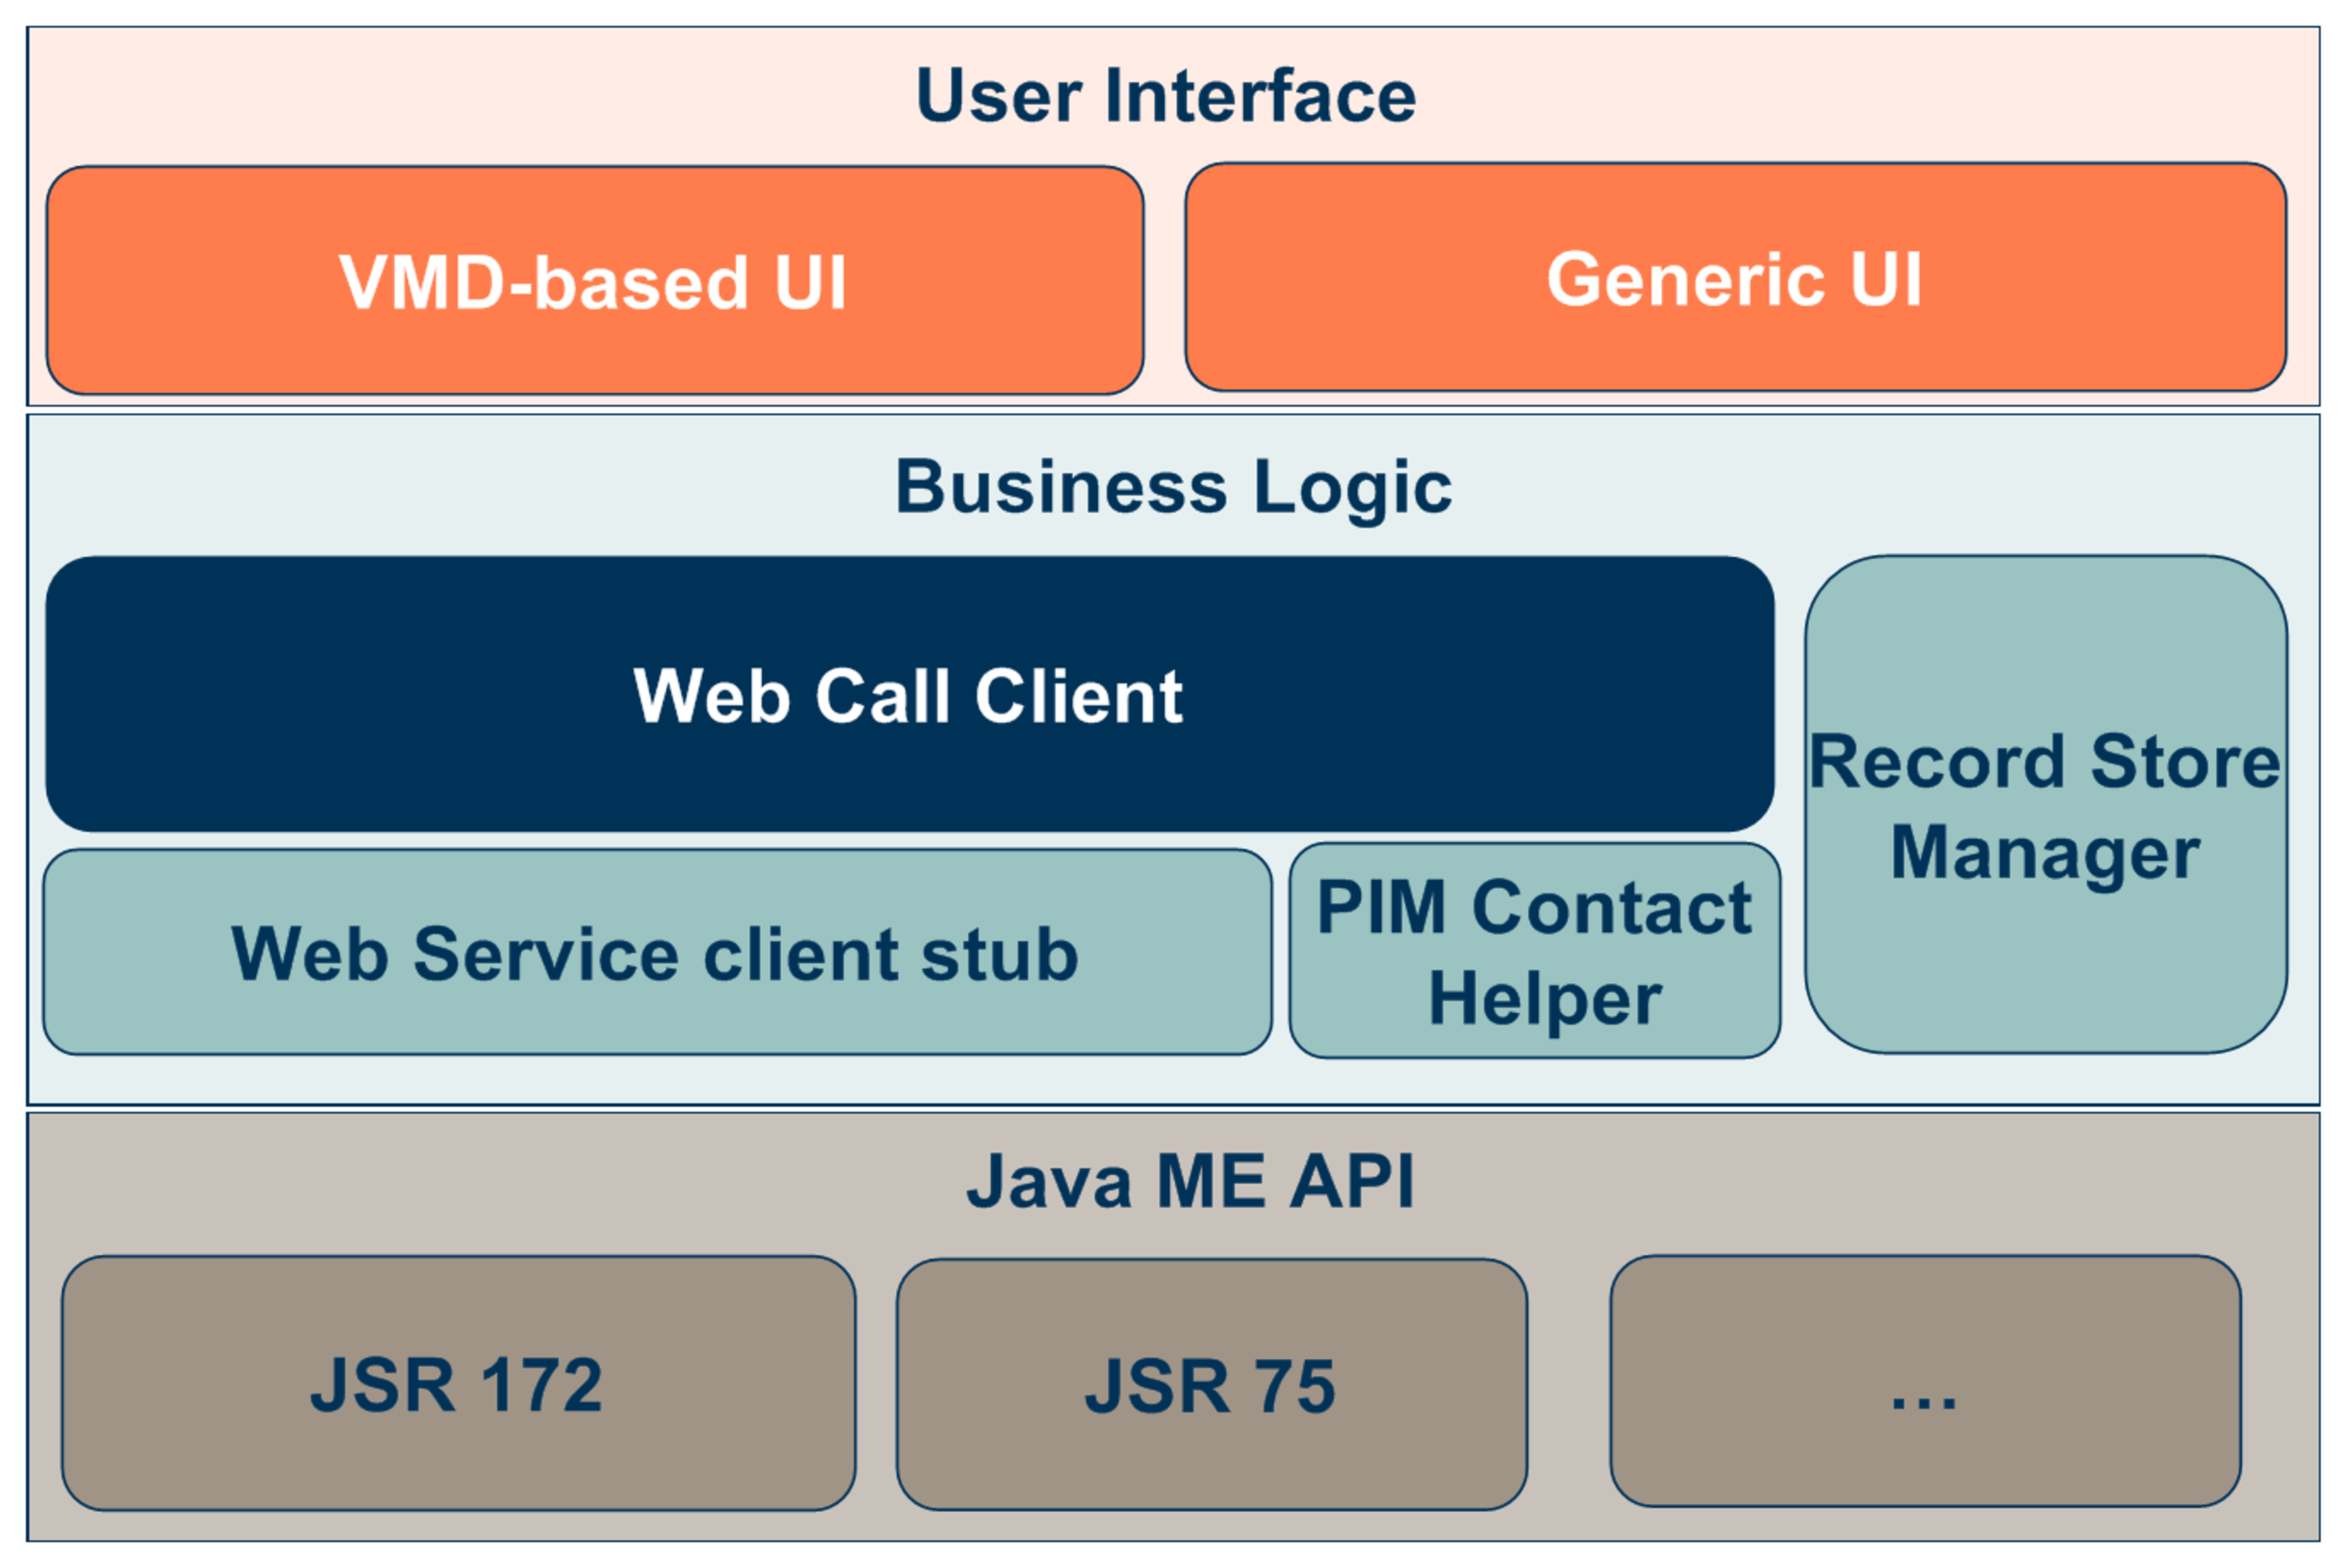
\epsfig{file=chap09/resources/java_me_client_architecture, width=5.2in}
\caption{The Architecture of Java ME Client}
\label{fig:TheArchitectureOfJavaMEClient}
\end{figure}


\section{Web Service Client Stub}
\label{sec:JavaMEClient:WebServiceClientStub}


\begin{figure}[!hbtp]
\centering
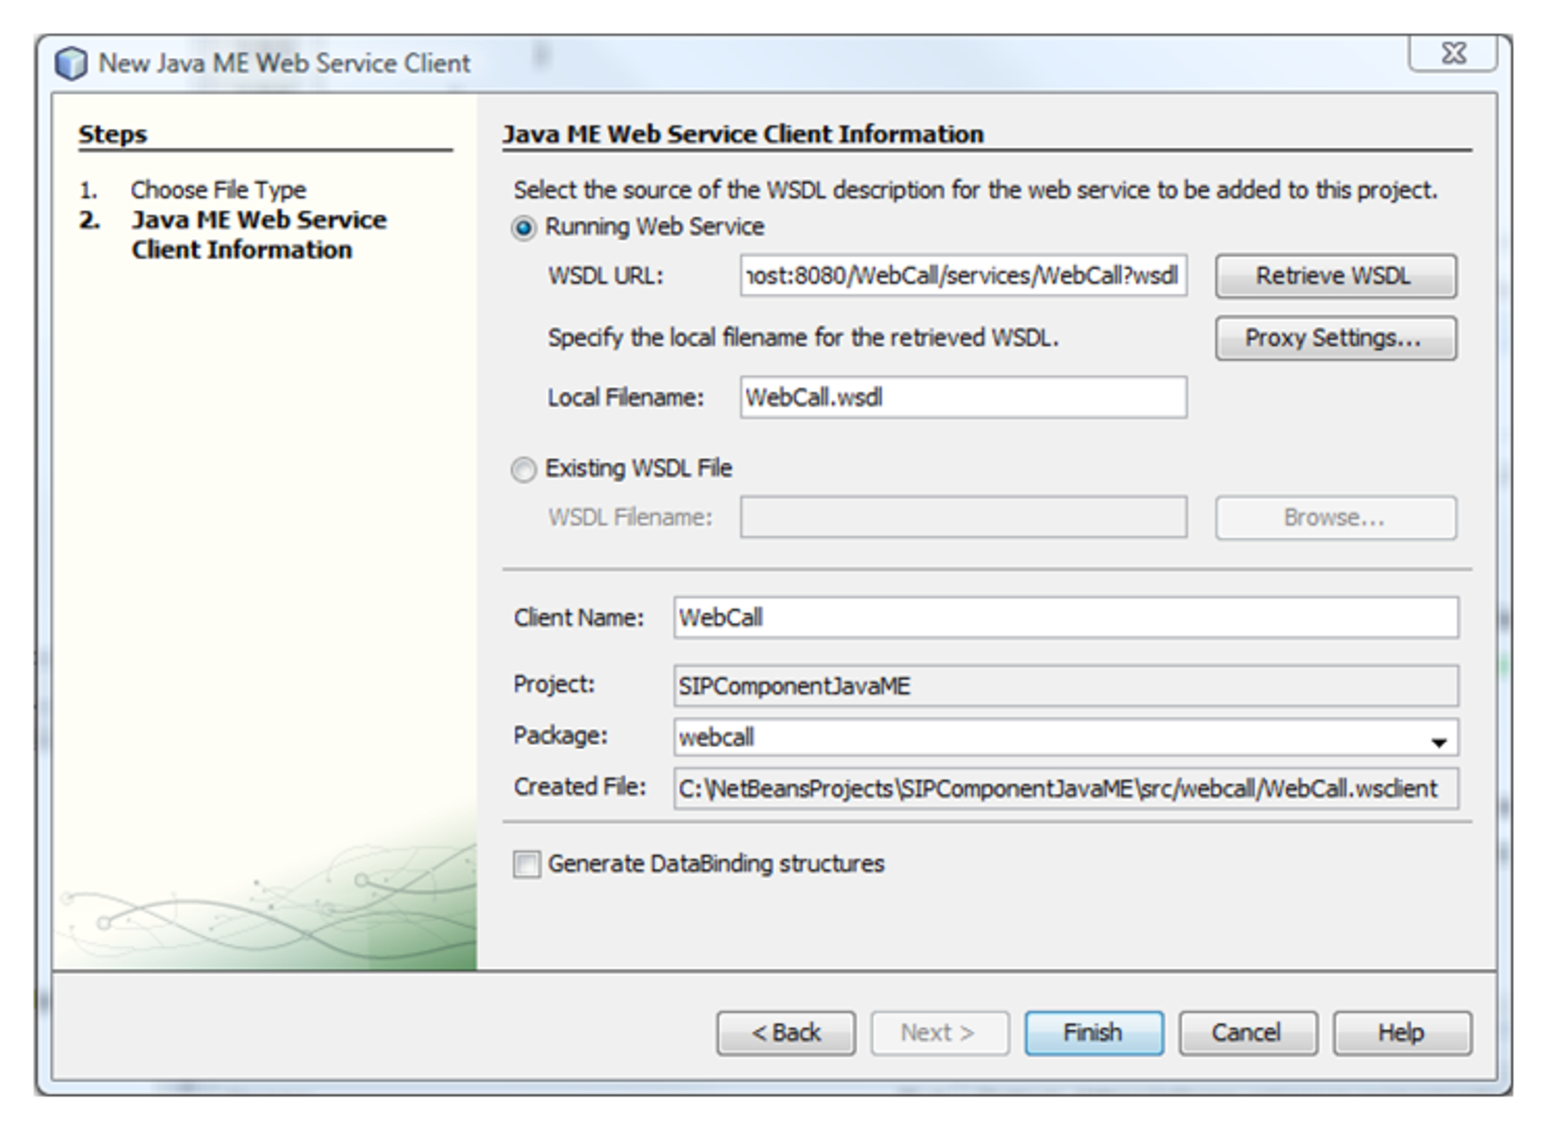
\epsfig{file=chap09/resources/Netbeans_Java_ME_Web_Service_Client_Wizard, width=5.2in}
\caption{Netbeans Java ME Web Service Client Wizard}
\label{fig:NetbeansJavaMEWebServiceClientWizard}
\end{figure}

\section{Record Store Manager}
\label{sec:JavaMEClient:RecordStoreManager}

\begin{figure}[!hbtp]
\centering
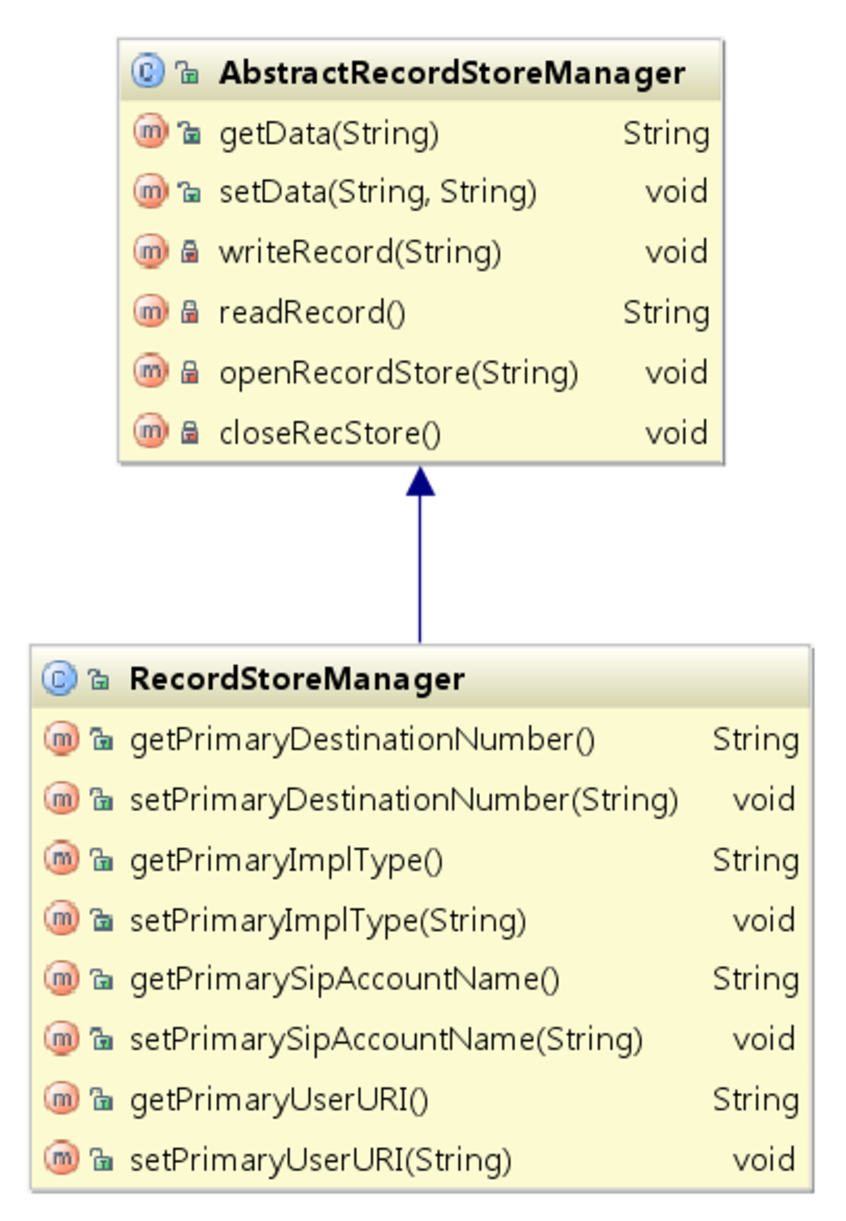
\epsfig{file=chap09/resources/record_store_manager, width=4in}
\caption{The Class Diagram of Record Store Manager}
\label{fig:TheClassDiagramofRecordStoreManager}
\end{figure}

\section{PIM Contact Helper}
\label{sec:JavaMEClient:PIMContactHelper}


\begin{figure}[!hbtp]
\centering
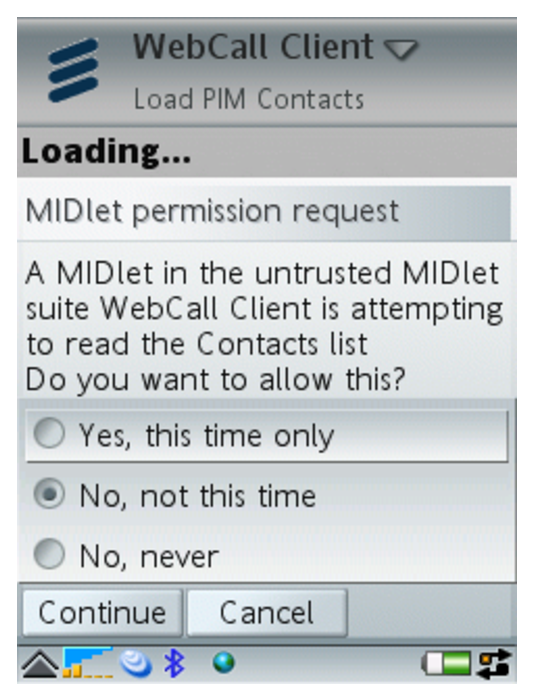
\epsfig{file=chap09/resources/load_pim_contacts, width=3in}
\caption{Load PIM Contacts}
\label{fig:Load PIM Contacts}
\end{figure}


\begin{figure}[!hbtp]
\centering
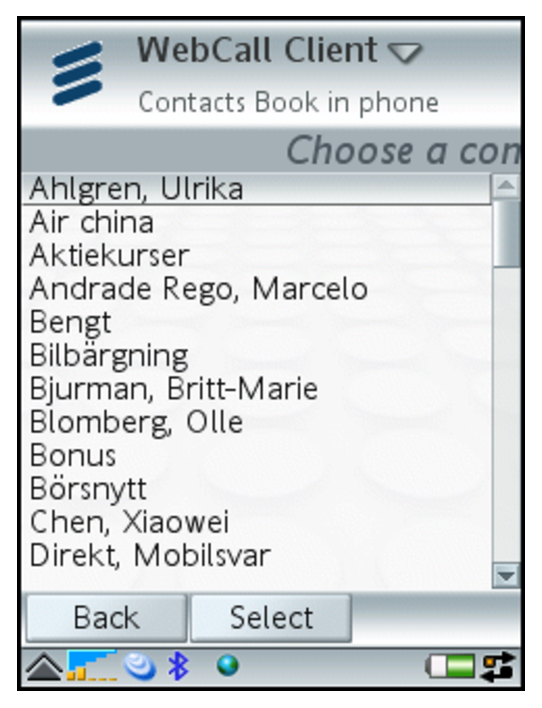
\epsfig{file=chap09/resources/pim_contacts, width=3in}
\caption{PIM Contacts List}
\label{fig:PIMContactsList}
\end{figure}

\section{Web Call Client}
\label{sec:JavaMEClient:WebCallClient}






\section{User Interface}
\label{sec:JavaMEClient:UserInterface}

\begin{figure}[!hbtp]
\centering
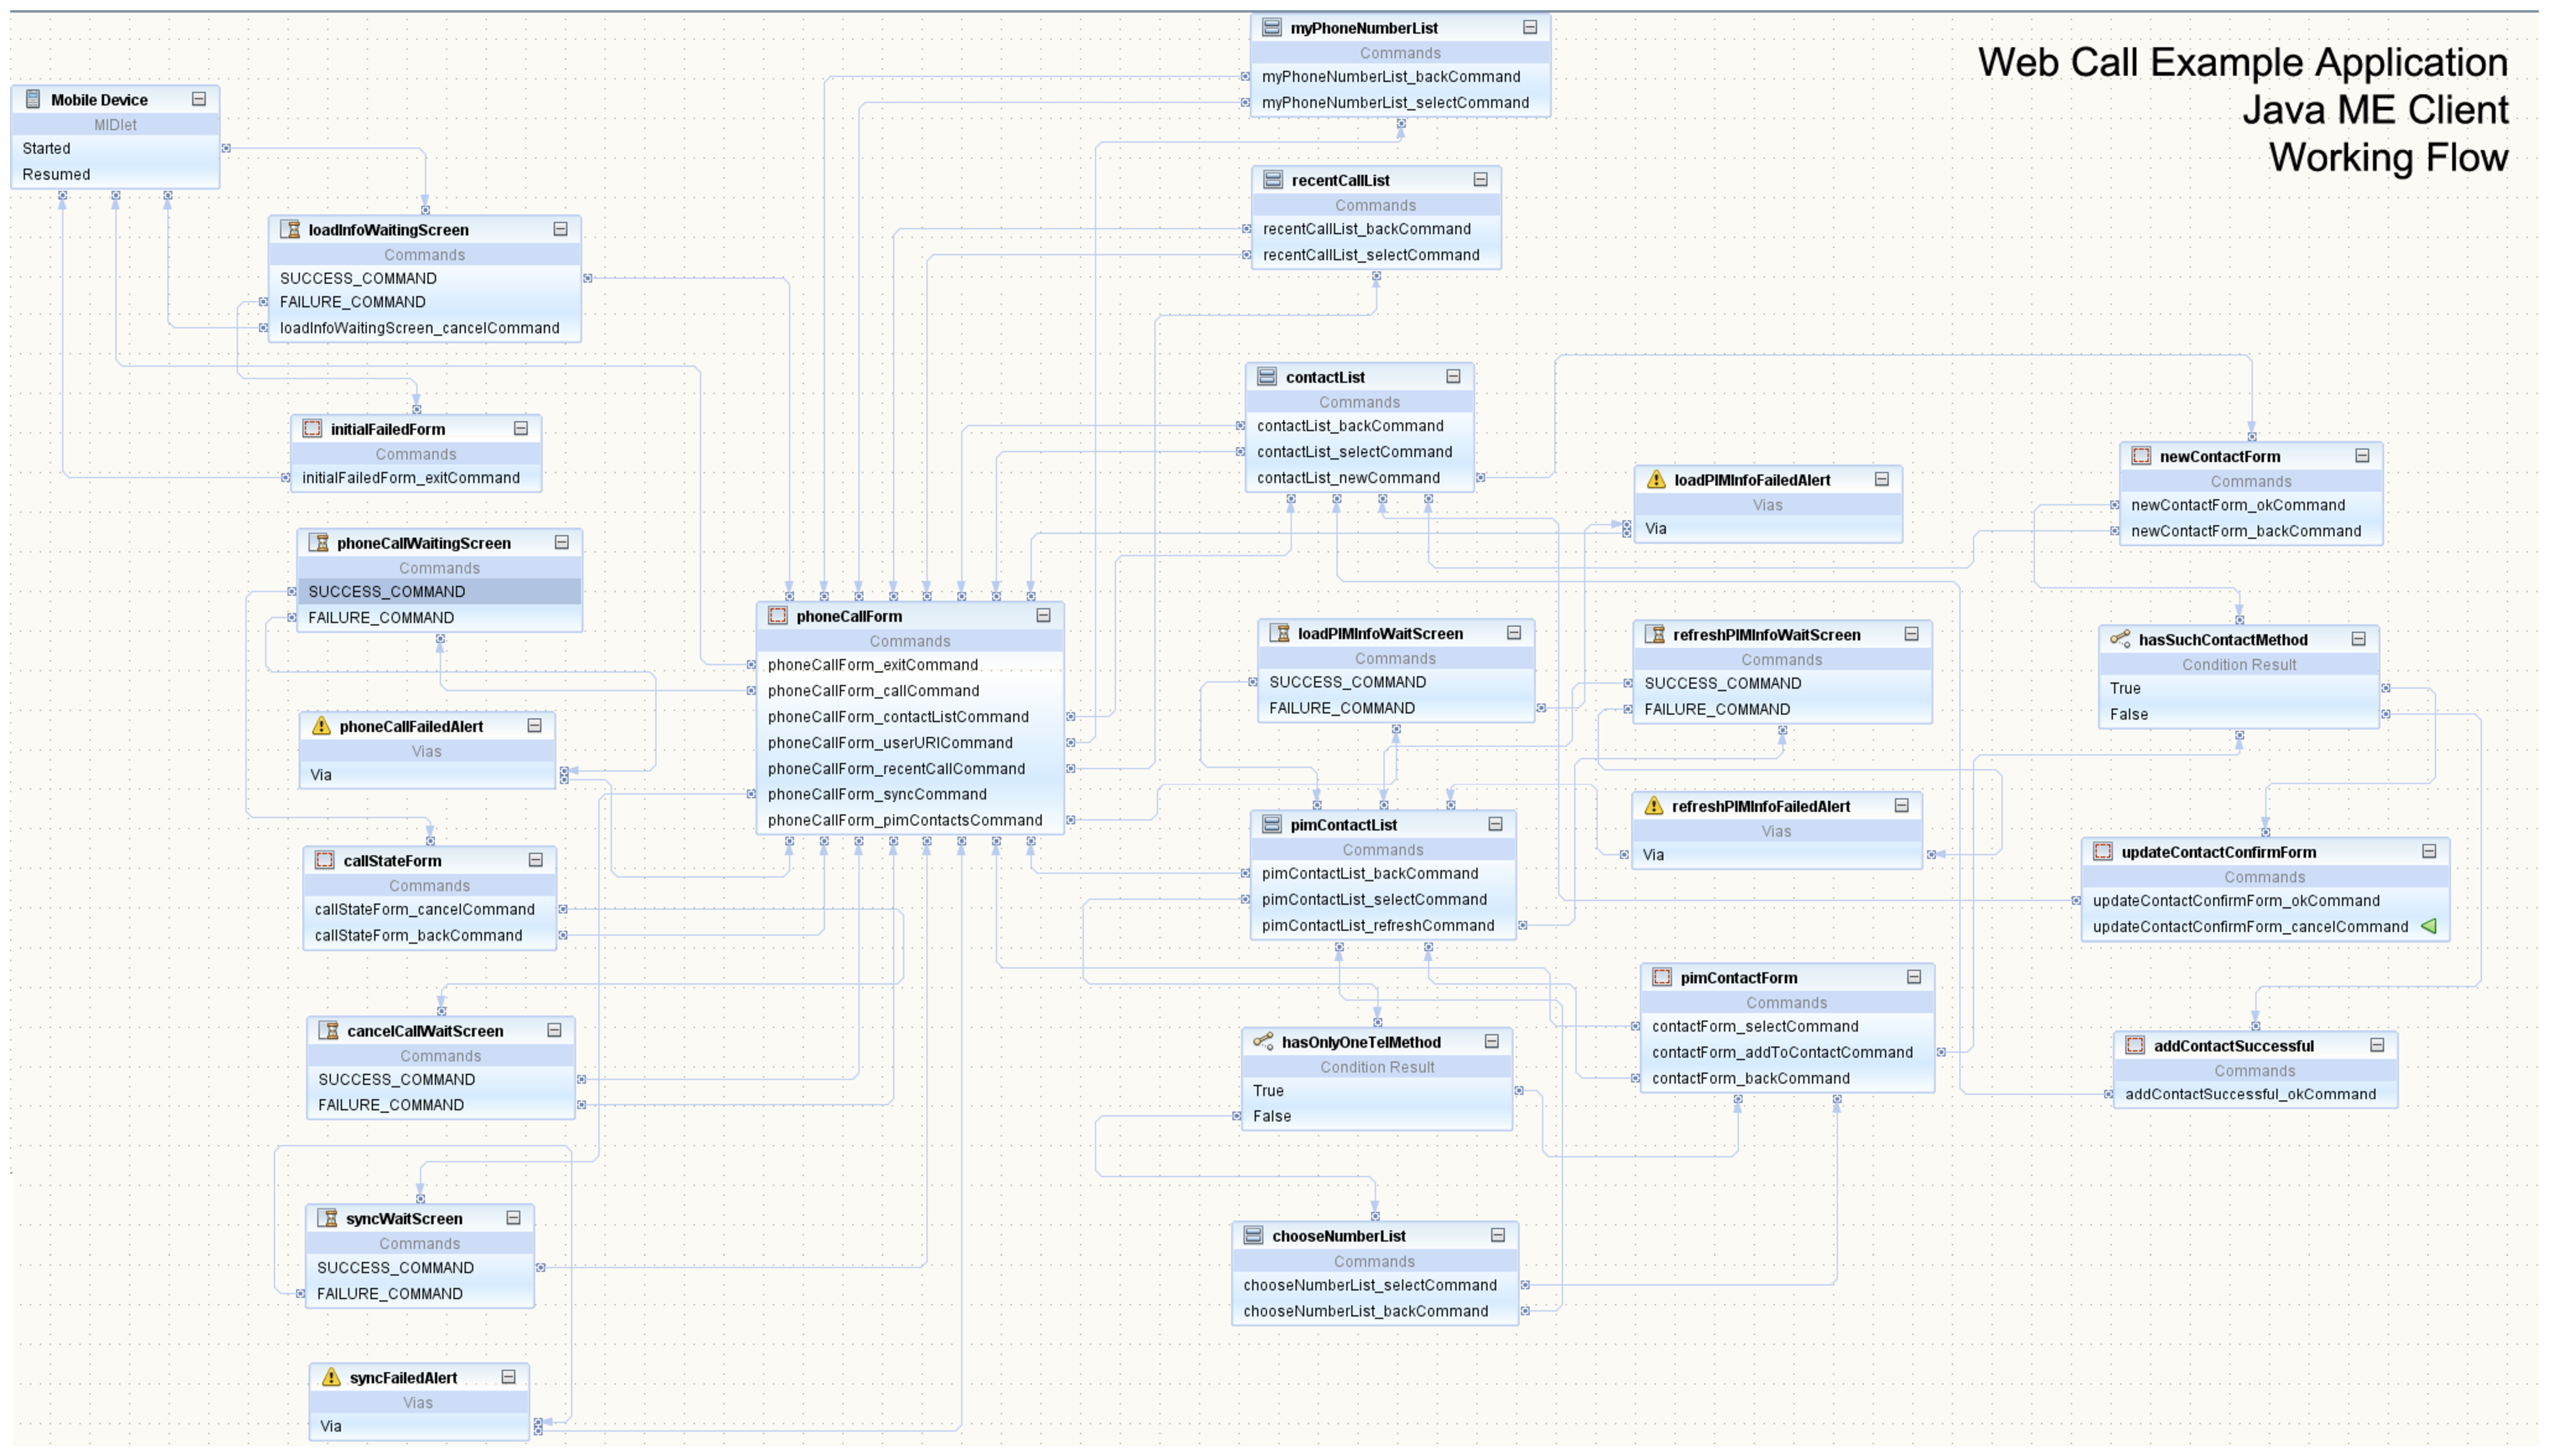
\epsfig{file=chap09/resources/java_me_working_flow, width=8.3in, angle=-90}
\caption{Java ME Client Working Flow}
\label{fig:JavaMEClientWorkingFlow}
\end{figure}

\subsection{VMD-based UI}
\label{sec:JavaMEClient:UserInterface:VMDBasedUI}



\subsection{Java ME Generic UI}
\label{sec:JavaMEClient:UserInterface:JavaMEGenericUI}

\section{Installation of Java ME Client}
\label{sec:JavaMEClient:InstallationOfJavaMEClient}

\section{Security of Java ME Client}
\label{sec:JavaMEClient:SecurityOfJavaMEClient}

% ********** End of chapter **********
